\documentclass[11pt,a4paper]{article}
\usepackage[utf8]{inputenc}
\usepackage[T1]{fontenc}
\usepackage[english]{babel}
\usepackage[margin=2.1cm]{geometry}
\usepackage{booktabs,array,tabularx}
\usepackage{xcolor}
\usepackage{graphicx}
\usepackage{pgfplots}
\pgfplotsset{compat=1.17}
\PassOptionsToPackage{hyphens}{url}
\usepackage[hidelinks]{hyperref}
\usepackage{enumitem}
\setlist{nosep,leftmargin=1.4em}
\emergencystretch=3em

\definecolor{impl}{HTML}{3B6EA8}
\definecolor{rev}{HTML}{8FB3DA}
\definecolor{waste}{HTML}{C8553D}

\title{Sweatshop on P-Chess: Stockfish analysis\\\large Stockfish 19 shipped (CI-004), a second engine on the UCI bridge (REV-001), game analysis (REV-002), move classification (REV-003) and accuracy (REV-004); GPT-6.1 Terra lineup, lane \texttt{analysis}}
\author{Foreman, session \texttt{sweatshop/analysis/2026-10-30-1831}}
\date{30 October 2026}

\begin{document}
\maketitle

\section*{Summary}

A lane run (\texttt{-Lane analysis}) in a fresh clone at \path{.artifacts-build/lanes/analysis},
default lineup \texttt{terra}: stage 2 on \texttt{gpt-6.1-terra high} for the two
\texttt{normal} tickets and \texttt{gpt-6.1-terra xhigh} for the three \texttt{hard} ones; review
on \texttt{gpt-6.1-sol xhigh}. The lanes \texttt{repertoire} and \texttt{v010} ran at the same time
in their own clones. Launch at 18:31, relaunch at 19:03 after a proxy answer, the five planned
tickets merged by 20:08; a third launch at 20:28 ran a follow-up (CLEAN-009) for the session PR's
red Linux CI, merged at 20:36.

\begin{itemize}
  \item \textbf{Produced:} CI-004, REV-001, REV-002, REV-003, REV-004 and the follow-up CLEAN-009
        merged on the session, all \texttt{Verdict: Approve} (CI-004 and REV-003
        \texttt{Review: human}, the others \texttt{Review: agent}). Session PR
        \href{https://github.com/Laginho/P-Chess/pull/26}{\#26}, checks green (Linux
        \texttt{test} 306/0, \texttt{windows-export}). Gate 306 passed, 0 failed, 0 skips (270 on
        \texttt{main} at launch).
  \item \textbf{Cost:} \textbf{\$6.31} at API list price over the 8 priced stages: \$6.15 for the 7
        \texttt{gpt-6.1-sol xhigh} reviews, \$0.16 for CLEAN-009's \texttt{gpt-6.1-terra high}
        stage (the driver priced Terra from its 20:28 launch); the other 9 Terra stages log
        \texttt{?}. Codex quota: 7 points of the weekly window (Terra high 1, Terra xhigh 3, Sol
        xhigh 3, outside stages 0; each $\pm$1), shared with the two concurrent lanes.
  \item \textbf{What went wrong:} CI-004 burned two stage-2 attempts and was parked
        \texttt{blocked}. The first ran the gate with a Godot it downloaded itself, after failing to
        find the installed one; Godot could not write \texttt{user://}, child processes
        multiplied, the gate was killed. The second stopped in a minute, reading the saved attempt as
        an interrupted \texttt{implementing}. The foreman put it to the proxy; the third attempt took
        3~minutes. REV-003 was reopened once with three findings (two P2). And the session PR's
        Linux \texttt{test} check was red from REV-001's merge to CLEAN-009's: two bridge tests faked
        a live engine with the test's own pid, which Linux rejects. The Windows gate and both reviews
        passed them; the foreman only looked at the PR's checks after the five tickets merged.
  \item \textbf{Provisional verdict:} on real feature work Terra was fast (median 6~min per
        to-review stage 2) and disciplined (red$\to$green on every behaviour, two mutation checks),
        and it asked the right question on REV-002. It struggled when the environment did not
        behave and no instruction covered it, and its test fakes were not portable. Its pair with
        Sol xhigh as reviewer now has 12 reviews for Terra high (25\% reopened) and 5 for Terra
        xhigh.
\end{itemize}

\section*{What was done}

\textbf{CI-004}: \path{scripts/fetch-engine.ps1} now also downloads the pinned official
Stockfish 19 Windows build, checks the SHA-256 of the archive and of the installed exe, and puts
\path{engine/stockfish/stockfish.exe} and its \texttt{Copying.txt} beside Lc0; a second run
downloads nothing. The release zip ships both, and \path{docs/THIRD_PARTY.md} gains a Stockfish
section. Not reopened. The two failed attempts were environment and state handling, not code (see
Driver and runtime issues).

\textbf{REV-001}: the UCI bridge (\path{engine/uci.gd}) takes a configurable engine and path, so a
second engine can run beside Maia's Lc0, and forwards every search \texttt{info} line and
\texttt{bestmove} to the caller. Maia's behaviour is unchanged. Merged with no finding.

\textbf{REV-002}: a new \path{engine/analyser.gd} runs Stockfish over every position of a saved
game, last to first, MultiPV 2, 3\,000\,000 nodes per position with an early stop once the best
move and score settle, and writes \path{user://analysis/<game>.json} with both lines, the best
move, terminal scores, the engine version and the budget; a file from another version or budget
reads as stale. \path{scripts/analyse.gd} does it headless for one PGN. The proxy approved two
small additions to the bridge for it (the handshake's \texttt{id name}, and \texttt{stop} during a
search). Merged with no finding. The foreman's probe on one of Bruno's saved games (124
positions) took 21.4~s.

\textbf{REV-003}: a new \path{core/classification.gd} grades each move (Forced, Repertoire, Book,
Brilliant, Great, Best, Excellent, Good, Inaccuracy, Mistake, Blunder, plus Miss, the lenient
Blunder and mate rules), with every threshold in \path{core/tunables.gd}. Reopened once: a capture
right after a pawn push was taken for a recapture (only the destination squares were compared), so
it lost Great; a free en passant capture got Great because the empty destination square hid the
victim; and one 0~cp cutoff stayed a literal outside \path{core/tunables.gd}. All three in
\path{core/classification.gd}, all fixed test-first in one pass.

\textbf{REV-004}: a new \path{core/accuracy.gd} gives each move's accuracy and each side's game
accuracy with Lichess's published formula. Tested against two real Lichess games, matching the
site's figures (87/94 and 85/72). Merged with no finding.

\textbf{CLEAN-009} (follow-up written by the foreman, triaged by the proxy): nothing changes for the
player. Three bridge tests in \path{tests/test_uci.gd} pretended an engine was running by giving the
bridge the test's own process id. Windows accepts that; Linux only tracks its own child
processes, so the bridge saw a stopped engine and two tests failed on CI from REV-001's merge on.
The tests now start a real idle Godot child (\path{tests/fixtures/idle_child.gd}), as the runner's
own tests already did. Proven red on Windows by mutating the bridge, green on Linux CI (306/0).
\section*{Timeline}

\begin{tabularx}{\linewidth}{@{}lX@{}}
\toprule
18:29 & Clone of \texttt{origin} at \texttt{eea8c16}; gate in the clone 270/0. \texttt{main}'s CI on \texttt{eea8c16} still running (later green). \\
18:31 & Launch, pid 11396. Codex sessions cannot reach the proxy (the driver asks for them). \\
18:46 & CI-004 attempt 1 fails (14~min): code done, gate killed at 198/72 with a downloaded Godot. \\
18:47 & CI-004 attempt 2 stops in 1~min; parked \texttt{blocked} after two attempts. REV-001 stage 2. \\
18:53 & REV-001 to review (Terra high, 6~min). \\
18:59 & REV-001 merged, 0 findings. Nothing runnable (REV-002 needs CI-004); PR \#26 opened. \\
19:00 & Foreman asks the proxy about CI-004: resume from attempt 1's commit; \texttt{c748352}. \\
19:03 & Relaunch, pid 22892; Codex sessions now reach the proxy directly. \\
19:07 & CI-004 to review (Terra high, 3~min). \\
19:12 & CI-004 merged, 0 findings. REV-002 stage 2 (Terra xhigh). \\
19:17 & REV-002 stops to ask (scope of \path{engine/uci.gd}); its own proxy call fails; the driver asks. \\
19:19 & Proxy decides: two seams on the bridge. REV-002 stage 2 again. \\
19:30 & REV-002 to review (11~min). \\
19:35 & REV-002 merged, 0 findings. REV-003 stage 2. \\
19:44 & REV-003 to review (9~min). \\
19:48 & REV-003 reopened, 3 findings. Stage 2 again. \\
19:52 & REV-003 to review (4~min). \\
19:56 & REV-003 merged. REV-004 stage 2. \\
20:04 & REV-004 to review (8~min); Codex then ends on ``model at capacity'', after the handoff commit. \\
20:08 & REV-004 merged; nothing left in the lane; PR \#26 updated (5 tickets). \\
20:19 & Foreman finds PR \#26's Linux \texttt{test} check red since 7940566 (304/2, \path{tests/test_uci.gd}). \\
20:23 & Proxy triages the foreman's follow-up CLEAN-009: tests only, a real child process. \\
20:28 & Third launch, pid 26744 (driver now prices Terra). \\
20:32 & CLEAN-009 to review (Terra high, 4~min). \\
20:36 & CLEAN-009 merged, 0 findings; PR \#26 updated (6 tickets). \\
20:38 & PR \#26's Linux \texttt{test} check green, 306/0. \\
\bottomrule
\end{tabularx}

\section*{Per stage}

{\small
\begin{tabularx}{\linewidth}{@{}llllrrrrrX@{}}
\toprule
When & Ticket & Stage & Model & Min & In & Cache & Out & Cost & Outcome \\
\midrule
18:46 & CI-004 & impl & terra high & 14 & 5.4M & 98\% & 12k & ? & failed \\
18:47 & CI-004 & impl & terra high & 1 & 0.2M & 88\% & 1k & ? & blocked \\
18:53 & REV-001 & impl & terra high & 6 & 2.9M & 97\% & 9k & ? & to-review \\
18:59 & REV-001 & review & sol xhigh & 6 & 2.8M & 95\% & 15k & 0.95 & merged \\
19:07 & CI-004 & impl & terra high & 3 & 1.3M & 96\% & 3k & ? & to-review \\
19:12 & CI-004 & review & sol xhigh & 5 & 2.5M & 96\% & 13k & 0.84 & merged \\
19:17 & REV-002 & impl & terra xhigh & 5 & 2.1M & 97\% & 6k & ? & asked \\
19:30 & REV-002 & impl & terra xhigh & 11 & 7.7M & 99\% & 26k & ? & to-review \\
19:35 & REV-002 & review & sol xhigh & 4 & 3.0M & 94\% & 14k & 1.04 & merged \\
19:44 & REV-003 & impl & terra xhigh & 9 & 5.9M & 98\% & 25k & ? & to-review \\
19:48 & REV-003 & review & sol xhigh & 4 & 3.1M & 95\% & 15k & 1.07 & reopened \\
19:52 & REV-003 & impl & terra xhigh & 4 & 2.3M & 97\% & 7k & ? & to-review \\
19:56 & REV-003 & review & sol xhigh & 4 & 2.2M & 93\% & 11k & 0.85 & merged \\
20:04 & REV-004 & impl & terra xhigh & 8 & 6.1M & 98\% & 16k & ? & to-review \\
20:08 & REV-004 & review & sol xhigh & 4 & 2.3M & 94\% & 13k & 0.85 & merged \\
20:32 & CLEAN-009 & impl & terra high & 4 & 1.6M & 97\% & 6k & 0.16 & to-review \\
20:36 & CLEAN-009 & review & sol xhigh & 4 & 2.0M & 94\% & 12k & 0.55 & merged \\
\midrule
 & & & & 96 & 53.4M & & 204k & 6.31+? & \\
\bottomrule
\end{tabularx}
}

\begin{center}
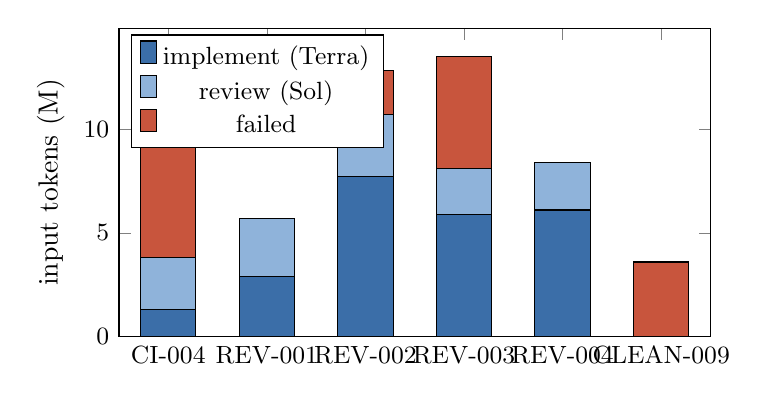
\begin{tikzpicture}
\begin{axis}[ybar stacked, bar width=20pt, width=0.75\linewidth, height=5.5cm,
  symbolic x coords={CI-004,REV-001,REV-002,REV-003,REV-004,CLEAN-009},
  xtick=data, ylabel={input tokens (M)}, ymin=0, legend style={at={(0.02,0.98)},anchor=north west,font=\small},
  tick label style={font=\small}]
\addplot[fill=impl] coordinates {(CI-004,1.3) (REV-001,2.9) (REV-002,7.7) (REV-003,5.9) (REV-004,6.1) (CLEAN-009,0)};
\addplot[fill=rev] coordinates {(CI-004,2.5) (REV-001,2.8) (REV-002,3.0) (REV-003,2.2) (REV-004,2.3) (CLEAN-009,0)};
\addplot[fill=waste] coordinates {(CI-004,5.6) (REV-001,0) (REV-002,2.1) (REV-003,5.4) (REV-004,0) (CLEAN-009,3.6)};
\legend{implement (Terra), review (Sol), failed, asked or reopened rounds}
\end{axis}
\end{tikzpicture}
\end{center}

The chart is input tokens, not dollars: most Terra stages are unpriced. Red: CI-004's two failed
attempts (5.6M; attempt 1's code was reused, so only its gate run and attempt 2 were lost),
REV-002's asking attempt (2.1M, a legitimate question, not a defect), REV-003's first review
plus fix round (3.1M + 2.3M), and all of CLEAN-009 (1.6M + 2.0M, the repair of REV-001's and
REV-002's non-portable tests).

\section*{Comparison with previous runs}

From \texttt{run-log.md}: over its P-Chess runs, \texttt{gpt-6.1-sol high} took a median of about
11~minutes per stage 2 and \texttt{gpt-6.1-sol xhigh} 11--22 on hard tickets, at \$0.4--1.5 per
stage. This run's Terra stage 2s that reached review took 3--11~minutes (median 6): 6, 3 and 4 on
the normal tickets, 11, 9 and 8 on the hard ones. Reviews cost what they did before
(\$0.55--1.07 against \$0.75--1.26). The repertoire and v010 lanes, run in parallel on the same
lineup, saw the same speed and a related weak spot: tickets stalled on environment or handoff
hygiene, not on the code.

\section*{Observations per model}

\begin{itemize}
  \item \textbf{gpt-6.1-terra high, stage 2} (5 stages, CI-004, REV-001 and CLEAN-009): REV-001
        looked clean (red, green, a second red/green for search forwarding, a mutation run, gate
        274/0 in 6~minutes), but its fake engine used the test's own pid, which only Windows
        accepts; REV-002 copied the pattern. Only Terra commits use it
        (\texttt{git log -S "OS.get\_process\_id()" -- tests/}); Sol's earlier bridge tests ran a
        real Lc0 and skipped without it. CLEAN-009, with the proxy's recipe, fixed it in 4~minutes
        with the mutation reds the ticket asked for. CI-004's code was right the first time, but the stage handled the environment
        badly: it did not find \texttt{godot} (REV-001's session, in the same sandbox, found it
        through \texttt{where.exe} and the profile), downloaded Godot from GitHub instead, and
        then read the global ``re-run the gate only after a code change'' rule as ``the gate
        cannot run again''. Attempt 2 refused to start because the saved attempt's ticket text
        said \texttt{implementing}, although the session's copy said \texttt{to-implement}. With
        the proxy's explicit recipe the third attempt was flawless.
  \item \textbf{gpt-6.1-terra xhigh, stage 2} (5 stages, the hard tickets): stopped at the right
        place on REV-002 (a seam the ticket did not name), with a precise question; then 11
        alternating test/production commits, +574 lines in scope. REV-003 and REV-004: one
        \texttt{test:} commit before every behaviour, a self-corrected test expectation verified
        red first, a mutation check on REV-004, and real Lichess games as fixtures. Missed: chess
        edge cases in its own exclusion logic (recapture, en passant) and one threshold left out
        of the tunables file. On REV-003 it noticed that criterion 7's ``+600~cp after'' branch
        cannot be reached under the clamped formula and documented it instead of asking; the
        reviewer agreed. One commit-hygiene slip: the P3 fix rode in the en passant commit.
  \item \textbf{gpt-6.1-sol xhigh, review} (7 stages, 4--6~min): verified receipts and red/green
        order, re-checked CI-004's hashes against the official release, and reproduced both
        REV-003 P2s with an external probe. The re-review raised nothing new (no drip-feed). No
        production code written in review, so no round-0 rows. Its 4-minute pass over REV-002's
        +574 lines found nothing; the foreman's real-game probe agrees with it. It reused the
        Windows gate receipt every time and never looked at the session PR's Linux check, so it
        approved REV-002 while that check was already red (review miss on the copied fake-pid
        test). CLEAN-009's review flagged the Linux confirmation as pending for the foreman.
\end{itemize}

\section*{Driver and runtime issues}

\begin{enumerate}
  \item \texttt{\$CodexPrices} had no \texttt{gpt-6.1-terra} row for the first two launches: 9
        Terra stages log \texttt{?}. The driver at the 20:28 launch (SHA256 \texttt{5C16FF\ldots},
        changed locally between launches) priced CLEAN-009's stage at \$0.157.
  \item The session PR's Linux \texttt{test} check was red from 7940566 (REV-001's close, about
        19:00) until aad8460 (20:38). The driver pushes the session and moves on; no stage and no
        review reads the PR's checks, and the foreman only looked after the five tickets merged.
        Every gate in the loop runs on Windows, CI runs on Ubuntu.
  \item CI-004's sandbox gate: \texttt{make\_dir\_recursive} failures under \texttt{user://} with a
        Godot downloaded into \texttt{\%TEMP\%}, runner children timing out and spawning more
        Godots. The stage killed its own processes and the gate exited $-1$. The installed Godot
        passed the full gate in the same sandbox minutes later, so the stage's tool discovery was
        the cause, not the sandbox alone.
  \item Proxy reachability changed between launches: ``unreachable'' at 18:32, ``reached
        directly'' at 19:04. Yet REV-002's stage still got \texttt{ECONNREFUSED}, and Codex's
        automatic approval refused a networked retry (``could send repository context to an
        external service''). The driver's fallback (asking for it) worked.
  \item REV-004's Codex turn ended with ``Selected model is at capacity'' (exit 1, no final
        message), seconds after the handoff commit. The driver read the committed state
        correctly. Earlier in the stage, it would have cost an attempt.
  \item Tests share fixed-name files under \texttt{user://} (such as
        \texttt{test\_ui006\_settings.cfg} and \texttt{runner\_cases/}) across every clone, since the
        project name is the same. Concurrent lane gates could collide. Not observed this run.
  \item Shutdown 1.0--3.9~s per stage; no crash, no timeout. The driver started with ``local
        edits; not updated'' at all three launches.
\end{enumerate}

\section*{Recommendations}

\begin{enumerate}
  \item Watch the session PR's checks, not only the local gate: have the driver (or the foreman,
        at every finished stage) read the PR's \texttt{test} check after each push, and park the
        next ticket when it turns red. A Linux-capable gate (WSL, or a \texttt{Sync gate:} that
        runs the suite under the Linux Godot) would have caught the fake-pid tests at stage 2.
  \item Commit the driver change that prices \texttt{gpt-6.1-terra} (it ran only as a local edit);
        without it most Terra stages stay unpriced.
  \item Put the gate's Godot in the repo's bindings (or have \texttt{gate-evidence.ps1} resolve
        it) and say ``never download a toolchain'' in ticket-flow: Terra spent a 14-minute stage
        on a self-downloaded Godot.
  \item In ticket-flow, say that a saved recovery commit's \texttt{Stage:} is evidence, not
        state, and that ``re-run the gate only after a code change'' does not forbid a first
        complete run. Both misreadings came from rules, not from the code.
  \item For classification-like tickets, list the chess edge cases in the test list (en passant,
        captures after non-captures, promotions); Terra tested the named exclusions but not
        their edge cases.
  \item Keep Terra as the default for now: scoreboard row \texttt{gpt-6.1-terra high}
        $\rightarrow$ \texttt{gpt-6.1-sol xhigh} has 12 reviews (all three lanes), 3 reopened,
        S2 rate 25\%, against \texttt{gpt-6.1-sol high} $\rightarrow$ \texttt{gpt-6.1-sol xhigh}
        18 reviews, 22\% --- comparable. \texttt{gpt-6.1-terra xhigh} $\rightarrow$
        \texttt{gpt-6.1-sol xhigh} 5 reviews, 1 reopened, 20\% (an anecdote) against
        \texttt{gpt-6.1-sol xhigh} $\rightarrow$ \texttt{gpt-6.1-sol xhigh} 9 reviews, 11\%. The
        reopen rate does not count the two session-review findings, nor CI-004's two failed
        attempts and the repertoire lane's parked handoff; those are where Terra trails Sol.
\end{enumerate}

\section*{Human debt and proxy decisions}

No \texttt{Débito humano:} lines. Three \texttt{Proxy decided} lines, all by
\texttt{opus-5.5 xhigh} with receipts:

\begin{itemize}
  \item \textbf{CI-004} (asked by the foreman): ``Accept with one change: set CI-004 to
        \texttt{to-implement} and resume from \texttt{recovery/20261030-1847/CI-004} by
        cherry-picking only 423f2ed (drop aa2f15c entirely), then redo the manual check and run
        the gate once with the installed Godot -- the code is done and the only problems were the
        environment and the stale ticket text.''
  \item \textbf{REV-002} (asked by the driver): ``Approve widening \texttt{engine/uci.gd} and
        \texttt{tests/test\_uci.gd} by exactly two seams: the handshake's \texttt{id name}, and an
        in-search \texttt{stop}. -- Criteria 2, 5 and 6 can't be met without them. Spec §15.3 says
        Stockfish runs `through the same bridge as Lc0', and the REV-001 handoff already left
        these two paths to REV-002.''
  \item \textbf{CLEAN-009} (stage-1 triage asked by the foreman): ``Approve CLEAN-009 as written
        and run it now in the analysis session, at Difficulty normal with Review agent. Fix the
        tests only, by using a real child process; one engine/uci.gd seam is pre-approved as a
        fallback. The red proof comes from mutating production code on Windows, with CI run
        41143449186 cited as the cause.'' Stage 2 did not need the fallback seam.
\end{itemize}

\section*{Reopen attribution}

Labelled by the foreman (opus-5.5); the reviewer was \texttt{gpt-6.1-sol xhigh}, so no
self-judging. Rows appended to \path{.scratch/reopen-attribution.md}.

{\small\noindent
\begin{tabularx}{\linewidth}{@{}>{\raggedright\arraybackslash}p{1.6cm}X>{\raggedright\arraybackslash}p{2.7cm}X@{}}
\toprule
Ticket (round) & Finding & Label & Why \\
\midrule
REV-003 (1) & A capture after a pawn push taken for a recapture; loses Great & S2-explícito/\allowbreak código & criterion 5 names the recapture exclusion \\
REV-003 (1) & Free en passant capture gets Great (victim not on the destination square) & S2-explícito/\allowbreak código & criterion 5, free-piece exclusion \\
REV-003 (1) & 0~cp mate cutoff left as a literal & S2-explícito/\allowbreak código & criterion 9 (P3) \\
\midrule
\multicolumn{4}{@{}l}{\emph{After approval, discovery \texttt{session-review} (PR \#26's Linux \texttt{test} check)}} \\
REV-001 (--) & Bridge test fakes a live engine with the test's own pid; fails on Linux & S2-implícito ? & CI runs on Ubuntu and \path{tests/test_runner.gd} already uses a real child; review miss unknown (CI not visible yet) \\
REV-002 (--) & Second test copies the same fake; fails on Linux & S2-implícito ? & same cause; review miss yes (PR check already red at the review) \\
\bottomrule
\end{tabularx}
}

Ticket review totals: S2-explícito/código 3, S2-explícito/teste 0, S2-implícito 0, S1 0, S3-ruído 0;
no review miss, no review-induced churn, no fix made in review. Session review (counted apart, not
in the reopen rate): 2 findings, both S2-implícito ?, origins REV-001 \texttt{513acab} and REV-002
\texttt{8a79621}, both fixed by CLEAN-009 (\texttt{e40f327}, CI run 41145544373 306/0); one review
miss, one unknown. Copilot's review of PR \#26 did not run (quota). No release-audit or
post-release finding.

\section*{Scoreboard}

\texttt{scoreboard.ps1} over the ClassyCall, EasyMath, PhysiSyst, SIGAA-ME and SynchroNice main
checkouts, plus this lane's clone in place of P-Chess's main checkout (same merged run log; the
clone holds this run's attribution rows, which reach \texttt{main} with this report). It now holds
all three lanes of 30 October. Moved since the repertoire report (the v010 report came out between
this report's two versions): \texttt{gpt-6.1-terra high} 4 $\to$ 15 stage runs (1 $\to$ 3 failed:
CI-004 twice, OPEN-006 once; CLEAN-009 the first priced Terra stage, \$0.16), its pair with Sol
xhigh 3 $\to$ 12 reviews, 3 reopened, S2 rate 33\% $\to$ 25\%; new rows \texttt{gpt-6.1-terra
xhigh} (6 runs, 5 to review, 1 asked, median 9~min) and its pair (5 reviews, 1 reopened, S2 20\%);
session-review findings 28 $\to$ 30; \texttt{proxy-decision (opus-5.5 xhigh)} 4 (this lane 3,
the others 1). The other rows only changed order.

{\tiny
\begin{verbatim}
| Implementer | Stage runs | To review | Failed | Asked | Median min to review | Cost |
|---|---|---|---|---|---|---|
| gpt-6.1-sol high | 64 | 59 | 0 | 5 | 9m | $49.27 (64/64 priced) |
| opus-5.5 medium | 3 | 2 | 1 | 0 | 6m | $4.79 (3/3 priced) |
| opus-5.5 | 7 | 4 | 0 | 3 | 14m | $15.12 (7/7 priced) |
| gpt-6-luna max | 89 | 61 | 10 | 18 | 17m | $4.91 (85/89 priced) |
| sonnet-5.5 high | 2 | 2 | 0 | 0 | 7m | $3.77 (2/2 priced) |
| gpt-6-astra high | 1 | 0 | 0 | 1 | - | $3.92 (1/1 priced) |
| opus-5.5 xhigh | 18 | 14 | 4 | 0 | 12m | $91.78 (18/18 priced) |
| gpt-6.1-sol max | 6 | 5 | 0 | 1 | 24m | $12.12 (6/6 priced) |
| haiku-5.5 high | 2 | 0 | 2 | 0 | - | $1.00 (2/2 priced) |
| opus-5.5 high | 20 | 13 | 6 | 1 | 6m | $37.46 (20/20 priced) |
| gpt-6.1-sol xhigh | 9 | 9 | 0 | 0 | 12m | $9.84 (9/9 priced) |
| gpt-6.1-terra high | 15 | 12 | 3 | 0 | 7m | $0.16 (1/15 priced) |
| gpt-6.1-terra xhigh | 6 | 5 | 0 | 1 | 9m | ? |
| gpt-6-sol xhigh | 1 | 1 | 0 | 0 | 9m | $0.40 (1/1 priced) |
| fable | 1 | 1 | 0 | 0 | 11m | ? |
| gpt-6-luna | 8 | 4 | 4 | 0 | 37m | ? |
| gpt-6-sol | 6 | 5 | 1 | 0 | 17m | ? |
| gpt-5.6-sol | 5 | 4 | 1 | 0 | 17m | ? |
| gpt-6-astra | 18 | 11 | 6 | 1 | 8m | ? |
| sonnet | 5 | 3 | 2 | 0 | 14m | $10.53 (4/5 priced) |
| sonnet-5 xhigh | 11 | 6 | 2 | 3 | 8m | $18.09 (11/11 priced) |

| Implementer | Reviewer | Reviews | Reopened | Reopen rate | Reopened for S2 | S2 rate | Unclassified | Fixed in review for S2 |
|---|---|---|---|---|---|---|---|---|
| gpt-6.1-sol high | gpt-6.1-sol max | 38 | 12 | 32% | 9 | >=24% | 2 | 1 |
| opus-5.5 medium | gpt-6.1-sol max | 2 | 1 | 50% | 0 | >=0% | 1 | 0 |
| opus-5.5 | opus-5.5 | 4 | 0 | 0% | 0 | 0% | 0 | 0 |
| gpt-6-luna max | opus-5.5 high | 18 | 1 | 6% | 1 | 6% | 0 | 0 |
| gpt-6-luna max | gpt-6-sol max | 43 | 23 | 53% | 22 | 51% | 0 | 0 |
| ? | gpt-6-sol max | 1 | 0 | 0% | 0 | 0% | 0 | 0 |
| sonnet-5.5 high | gpt-6-sol max | 2 | 1 | 50% | 1 | 50% | 0 | 0 |
| opus-5.5 xhigh | gpt-6.1-sol max | 6 | 3 | 50% | 3 | 50% | 0 | 0 |
| ? | gpt-6.1-sol max | 1 | 0 | 0% | 0 | 0% | 0 | 0 |
| gpt-6.1-sol max | gpt-6.1-sol max | 4 | 1 | 25% | 1 | 25% | 0 | 0 |
| ? | opus-5.5 xhigh | 4 | 1 | 25% | 1 | 25% | 0 | 0 |
| opus-5.5 xhigh | opus-5.5 xhigh | 7 | 0 | 0% | 0 | 0% | 0 | 0 |
| opus-5.5 high | opus-5.5 xhigh | 10 | 2 | 20% | 2 | 20% | 0 | 3 |
| gpt-6.1-sol high | gpt-6.1-sol xhigh | 18 | 4 | 22% | 4 | 22% | 0 | 0 |
| gpt-6.1-sol xhigh | gpt-6.1-sol xhigh | 9 | 1 | 11% | 1 | 11% | 0 | 1 |
| gpt-6.1-terra high | gpt-6.1-sol xhigh | 12 | 3 | 25% | 3 | 25% | 0 | 0 |
| ? | gpt-6.1-sol xhigh | 1 | 0 | 0% | 0 | 0% | 0 | 0 |
| gpt-6.1-terra xhigh | gpt-6.1-sol xhigh | 5 | 1 | 20% | 1 | 20% | 0 | 0 |
| gpt-6-sol xhigh | gpt-6-astra high | 1 | 0 | 0% | 0 | 0% | 0 | 0 |
| fable | fable | 1 | 1 | 100% | 0 | >=0% | 1 | 0 |
| ? | opus | 1 | 0 | 0% | 0 | 0% | 0 | 0 |
| gpt-6-luna | gpt-6-sol | 4 | 4 | 100% | 0 | >=0% | 4 | 0 |
| gpt-6-sol | gpt-5.6-sol | 5 | 4 | 80% | 0 | >=0% | 4 | 0 |
| gpt-5.6-sol | gpt-6-astra | 4 | 3 | 75% | 0 | >=0% | 3 | 0 |
| gpt-6-astra | gpt-5.6-sol | 11 | 5 | 45% | 0 | >=0% | 5 | 0 |
| sonnet | opus | 3 | 1 | 33% | 1 | 33% | 0 | 0 |
| sonnet-5 xhigh | opus-5.5 xhigh | 5 | 0 | 0% | 0 | 0% | 0 | 0 |

| Implementer -> Reviewer | Rounds | S2 explicit code | S2 explicit test | S2 implicit | S1 | S3 noise |
|---|---|---|---|---|---|---|
| gpt-6-astra medium -> gpt-6.1-sol max | 8 | 11 | 1 | 4 | 1 | 0 |
| gpt-6.1-sol-fast high -> gpt-6.1-sol-fast max | 2 | 2 | 0 | 0 | 0 | 0 |
| gpt-6.1-sol-fast max -> gpt-6.1-sol-fast max | 6 | 2 | 0 | 3 | 1 | 0 |
| gpt-6.1-sol high -> gpt-6.1-sol max | 26 | 16 | 4 | 23 | 1 | 0 |
| gpt-6-luna max -> opus-5.5 high | 1 | 1 | 1 | 0 | 1 | 0 |
| gpt-6-luna max -> gpt-6-sol max | 23 | 31 | 3 | 23 | 12 | 15 |
| sonnet-5.5 high -> gpt-6-sol max | 1 | 3 | 0 | 2 | 0 | 0 |
| opus-5.5 xhigh -> gpt-6.1-sol max | 3 | 3 | 0 | 2 | 1 | 0 |
| gpt-6.1-sol max -> gpt-6.1-sol max | 5 | 7 | 0 | 5 | 0 | 0 |
| haiku-5.5 high -> gpt-6.1-sol max | 3 | 3 | 1 | 5 | 1 | 0 |
| gpt-6.1-sol high -> gpt-6.1-sol xhigh | 53 | 53 | 4 | 23 | 3 | 0 |
| gpt-6.1-sol max -> gpt-6.1-sol xhigh | 2 | 0 | 0 | 3 | 0 | 0 |
| opus-5.5 high -> opus-5.5 xhigh | 8 | 7 | 0 | 3 | 0 | 0 |
| gpt-6.1-sol xhigh -> gpt-6.1-sol xhigh | 3 | 4 | 0 | 1 | 0 | 0 |
| opus-5.5 high -> gpt-6.1-sol xhigh | 1 | 2 | 0 | 0 | 0 | 0 |
| gpt-6.1-terra high -> gpt-6.1-sol xhigh | 3 | 5 | 0 | 3 | 0 | 0 |
| gpt-6.1-terra xhigh -> gpt-6.1-sol xhigh | 1 | 3 | 0 | 0 | 0 | 0 |
| sonnet-5.5 high -> gpt-6.1-sol max | 3 | 5 | 0 | 2 | 3 | 0 |
| sonnet-5.5 xhigh -> gpt-6.1-sol max | 3 | 7 | 0 | 3 | 2 | 0 |
| sonnet-5.5 high -> opus-5.5 xhigh | 3 | 1 | 2 | 0 | 0 | 0 |
| gpt-6-astra medium -> gpt-6-astra xhigh | 1 | 1 | 0 | 0 | 0 | 0 |
| fable -> ? | 4 | 5 | 1 | 3 | 1 | 0 |
| sonnet -> ? | 10 | 3 | 6 | 9 | 3 | 2 |
| opus -> ? | 1 | 3 | 0 | 0 | 0 | 0 |
| sonnet? -> ? | 11 | 3 | 4 | 12 | 3 | 5 |
| sonnet -> opus | 1 | 1 | 1 | 0 | 0 | 0 |
| gpt-6-astra low -> gpt-6.1-sol max | 1 | 2 | 0 | 1 | 0 | 0 |

Evidence coverage: legacy flags and absent records are unknown, not zero defects or zero interventions.
| Discovery | Recorded findings | Earlier review miss (yes / known) | Review-induced churn (yes / known) |
|---|---|---|---|
| ticket-review | 375 | 5 / 180 | 1 / 182 |
| session-review | 30 | 23 / 25 | 0 / 29 |
| release-audit | 2 | 2 / 2 | 0 / 2 |
Runtime completion to process exit: 265.366s total over 212 measured stages; 334 unmeasured.
| Intervention | Recorded events |
|---|---|
| human-rescue | 30 |
| automatic-recovery | 89 |
| proxy-decision (unknown) | 37 |
| routine-approval | 18 |
| proxy-decision (gpt-6-astra high, fallback) | 58 |
| proxy-decision (opus) | 42 |
| proxy-decision (supervisor) | 12 |
| proxy-decision (opus-5.5 xhigh) | 4 |
\end{verbatim}
}

\section*{Acceptance}

The lane has no \texttt{spec.md} of its own, so no feature scenarios; the tickets' pending product
checks are in the PR. One was machine-checkable and the foreman ran it on the integrated session
(\texttt{8bb6467}): \path{scripts/fetch-engine.ps1} verified Stockfish 19, then
\path{scripts/analyse.gd} on a copy of Bruno's saved game \texttt{2026-10-26T23-21-19} analysed
124 positions in 21.4~s (exit 0): \texttt{engine\_version} ``Stockfish 19'',
\texttt{node\_budget} 3\,000\,000, two lines on 122 positions, one forced position with one line,
the final mate as a terminal score, PGN SHA-256 unchanged. Still Bruno's: classifications and
accuracy by eye on a real game once the review UI exists (REV-005, REV-006), and the tagged release
with Stockfish on a clean machine.

\section*{Pending for the human}

\begin{enumerate}
  \item Review and merge session PR \#26 (CI-004 and REV-003 are \texttt{Review: human}); its
        checks are green since CLEAN-009.
  \item After the merge, tell the \texttt{repertoire} and \texttt{v010} foremen to sync.
  \item Commit the driver's local edit that prices \texttt{gpt-6.1-terra}.
\end{enumerate}

\end{document}
